%
% Iniciando o documento
%
\documentclass[spectratio=169, portuguese]{beamer}
\usepackage[utf8]{inputenc}
\usepackage[brazil]{babel}
\usepackage[alf]{abntex2cite}	% Citações padrão ABNT
\usepackage{tikz}
\usepackage{graphicx}			% Inclusão de gráficos
\usepackage[T1]{fontenc}		% Selecao de codigos de fonte
%\usepackage[utf8x]{inputenc}	% Codificacao do documento (conversão automática dos acentos)
\usepackage{longtable}
\setlength{\LTpost}{0pt}
\setlength{\LTpre}{0pt}
\usepackage{pgfplots}
\pgfplotsset{compat=1.8}
\setbeamertemplate{caption}[numbered]
%
% Escolhendo o tema e seu esquema de cores
% 
\usetheme{PaloAlto}
\usecolortheme{crane}
%
% Inicia - Definir o slide mestre
%
\title{Usando o Trem Metropolitano da CPTM como fio-condutor para abordar questões territoriais na Grande São Paulo}
\author{
	Caio César Carvalho Ortega \\
	RA 21038515
	}
\date{\today}
%
% Inserindo um logotipo
% 
\titlegraphic{
\includegraphics[width=1.5cm]{logo_ufabc.png}\hspace*{0cm}
\logo{
\includegraphics[height=0cm]{logo_ufabc.png}}
}
%
% Conclui - Definir o slide mestre 
%
\begin{document}
\begin{frame}
\titlepage
\end{frame}
%
% A apresentação "de facto" começa a partir daqui
%

% ----------------- NOVO SLIDE --------------------------------
\section{Introdução}
\begin{frame}{A ideia}
	
	Mostrar algumas relações possíveis entre um recorte do território servido pelo Trem Metropolitano e conceitos abordados ao longo da disciplina.

\end{frame}
%%%
\begin{frame}{Do que vamos precisar?}

	\begin{itemize}
		\item Compreender o papel da CPTM
		\item Compreender o papel do Trem Metropolitano
		\item Identificar as relações em um recorte definido (ou seja, um pedaço da malha)
	\end{itemize}

\end{frame}

% ----------------- NOVO SLIDE --------------------------------

\begin{frame}{Certo! O que é a CPTM, afinal?}
	
	\begin{figure}[h]
		
\includegraphics[keepaspectratio,width=5cm]{beamer/cptm_logotipo.png}
	\end{figure}
	
	A CPTM é uma empresa estatal de economia mista, ligada à Secretaria dos Transportes Metropolitanos do Governo de Estado de São Paulo, criada em 28 de maio de 1992 por força da Lei Estadual nº 7.861\cite{sitecptm1}. O papel da empresa é definido no artigo 4º da mesma lei.
	
\end{frame}

% ----------------- NOVO SLIDE --------------------------------

\begin{frame}{1992: a lei}
		
	\begin{exampleblock}{}
		Artigo 4º -- A CPTM terá por objeto:\\
		I -- planejamento, estudo, projeto, construção, implantação, exploração e manutenção das obras e serviços de transporte de passageiros, sobre trilhos ou guiados, nas entidades regionais do Estado de São Paulo;\\
		II -- execução das obras e dos serviços complementares ou correlatos, necessários à integração do sistema de transporte por ela operado ao complexo urbanístico das cidades servidas pelo sistema; \\
		III --  operação de conexões intermodais de transporte de passageiros, no sistema por ela explorado, como terminais, estacionamentos e outras correlatas;\\		
		(\dots)
	\end{exampleblock}
	
\end{frame}

% ----------------- NOVO SLIDE --------------------------------

\begin{frame}{1992: a lei}
	
	\begin{exampleblock}{}
		IV -- prestação a terceiros de serviços de transporte de cargas, ou de passageiros, de passagem pelo território por ela servido;
		V -- comercialização de marca, patente, nome e insígnia; comercialização de áreas e espaços para propaganda; prestação de serviços complementares de suporte ao usuário, por si ou por meio de terceiros, com ou sem cessão de uso predial;\\
		VI -- comercialização de tecnologia, direta ou indiretamente, em sociedades ou em consórcios; prestação de serviços de consultoria, gerenciamento e apoio técnico; prestação de serviços de operação e manutenção de equipamentos; construção e implantação de sistemas de transporte e terminais de passageiros, no País ou no exterior; e\\
		VII -- edição de jornais, revistas e outras publicações de caráter técnico ou comercial.\cite{lei7861}
	\end{exampleblock}

\end{frame}

% ----------------- NOVO SLIDE --------------------------------

\begin{frame}{1993: a assembleia}
	
	Segundo \citeonline[p. 236]{Stefani}, ``a formação da CPTM tornou-se oficial após aprovação na Assembléia Geral da	Constituição, realizada em 02.07.1993, tendo como acionistas a Fepasa e a Companhia Metropolitana de Transportes Coletivos – CMTC''.
	
\end{frame}

% ----------------- NOVO SLIDE --------------------------------

\begin{frame}{Lei abrangente, papel impreciso}
	
	Vale notar que a CPTM possui um papel difuso, apontado por \citeonline[p. 122]{Isoda}: ``Em suma, a CPTM tem hesitado em definir quais os seus papéis no transporte metropolitano, abarcando simultaneamente as escalas metropolitana, regional, e central-metropolitana (em grande parte por omissão da CMSP)''. 
	
\end{frame}

% ----------------- NOVO SLIDE --------------------------------

\begin{frame}{Certo! E o Trem Metropolitano?}
	
	O Trem Metropolitano é o serviço ferroviário da CPTM (que transita entre as escalas mencionadas no slide anterior) que tem alta capacidade e opera por meio de seis linhas:

	\begin{itemize}
		\item 7 - Rubi (Luz-Francisco Morato-Jundiaí)
		\item 8 - Diamante (Júlio Prestes-Itapevi-Amador Bueno)
		\item 9 - Esmeralda (Osasco-Grajaú)
		\item 10 - Turquesa (Brás-Rio Grande da Serra)
		\item 11 - Coral (Luz-Guaianases-Estudantes)
		\item 12 - Safira (Brás-Calmon Viana)
	\end{itemize}
	
\end{frame}

% ----------------- NOVO SLIDE --------------------------------

\begin{frame}{Alta capacidade? É metrô então?}
	
	Conforme \citeonline{Isoda}[pág. 32], um serviço de alta capacidade é resumido como uma rede segregada e de linhas exclusivas; conforme \citeonline{Isoda}[pág. 51], ``Sistemas  de  alta  capacidade  operam  sempre  com  veículos  de  grande porte – composições de 4 a 12 carros, de 80 a 220 m de comprimento. Quanto  maior  o  veículo,  mais  pessoas  transportadas  por  vez,  maior capacidade.  Mas  quanto  maior,  mais  pesado,  maior  a  inércia,  o  que exige  mais  potencia  dos  motores,  além  de  maior  dificuldade  de aceleração e frenagem, reforçando a necessidade da segregação.''
	
\end{frame}

% ----------------- NOVO SLIDE --------------------------------

\begin{frame}{Linhas x Habitantes - Quadro}
	
	\begin{figure}[h]
		\caption{Quilometragem de rede por habitante \apud[p. 58]{Isoda}{Overden2009}
			\apud[p. 58]{Isoda}{Sort2005}}
		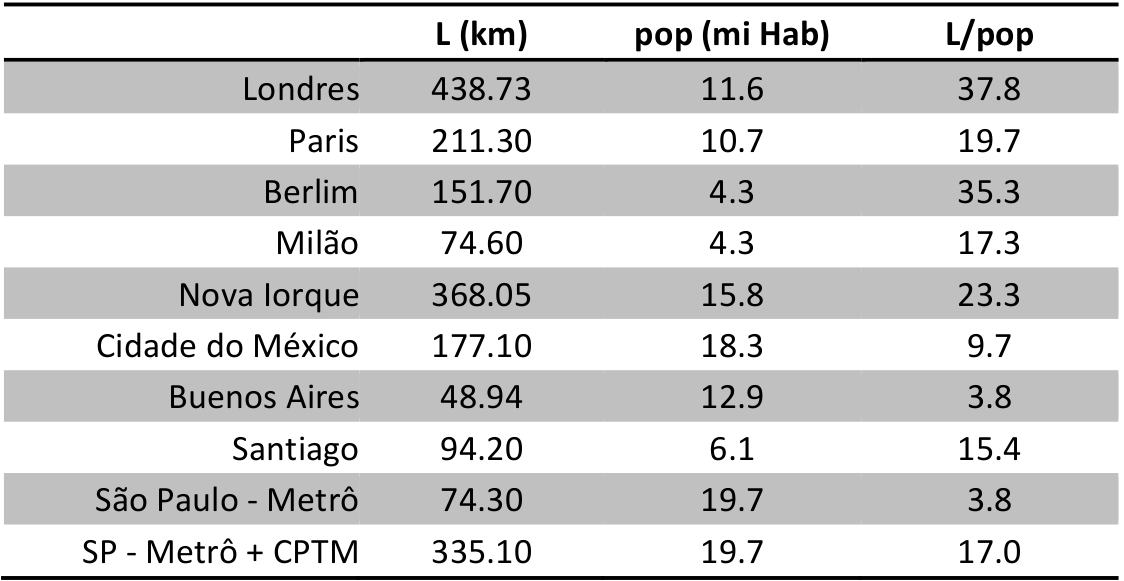
\includegraphics[keepaspectratio,width=\textwidth]{img_isoda_km_rede.png}
	\end{figure}

\end{frame}

% ----------------- NOVO SLIDE --------------------------------

\begin{frame}{Linhas x Habitantes - Melhor não ignorar a CPTM}
	
	\begin{alertblock}{Importante}
		Dissociar a rede da CPTM do território, acaba por eliminar um elemento estruturante importante, agravando o quadro de escassez de linhas por habitante, ao invés de induzir mudanças positivas.
		
		Para \citeonline[p. 16]{Ferreira} a presença da CPTM é marcante no território, com resultados entusiasmantes após mais de uma década de investimentos.
	\end{alertblock}

\end{frame}

% ----------------- NOVO SLIDE --------------------------------

\begin{frame}{Serviço em transformação}
	
	Em relação às redes conceituadas como metrô e surgidas em meados do século XIX, \citeonline[pág. 30]{Isoda} explica que estas malhas ``Não se diferenciavam tecnológica e operacionalmente das estradas de ferro  existentes,  com  grande  número  de  ramais  e  trechos  de  via compartilhada. Eram linhas independentes, de companhias diversas, e muitas  vezes  buscavam  apenas  conectar  estações  terminais  centrais das ferrovias que não conseguiam penetrar nos centros antigos \apud{Isoda}{Sort2005}'', 

\end{frame}

% ----------------- NOVO SLIDE --------------------------------

\begin{frame}{Retomando! Mapa da rede}
	
	\begin{figure}[h]
		\caption{Adaptação do mapa da rede, com as 92 estações \cite{sitecptm2}}
		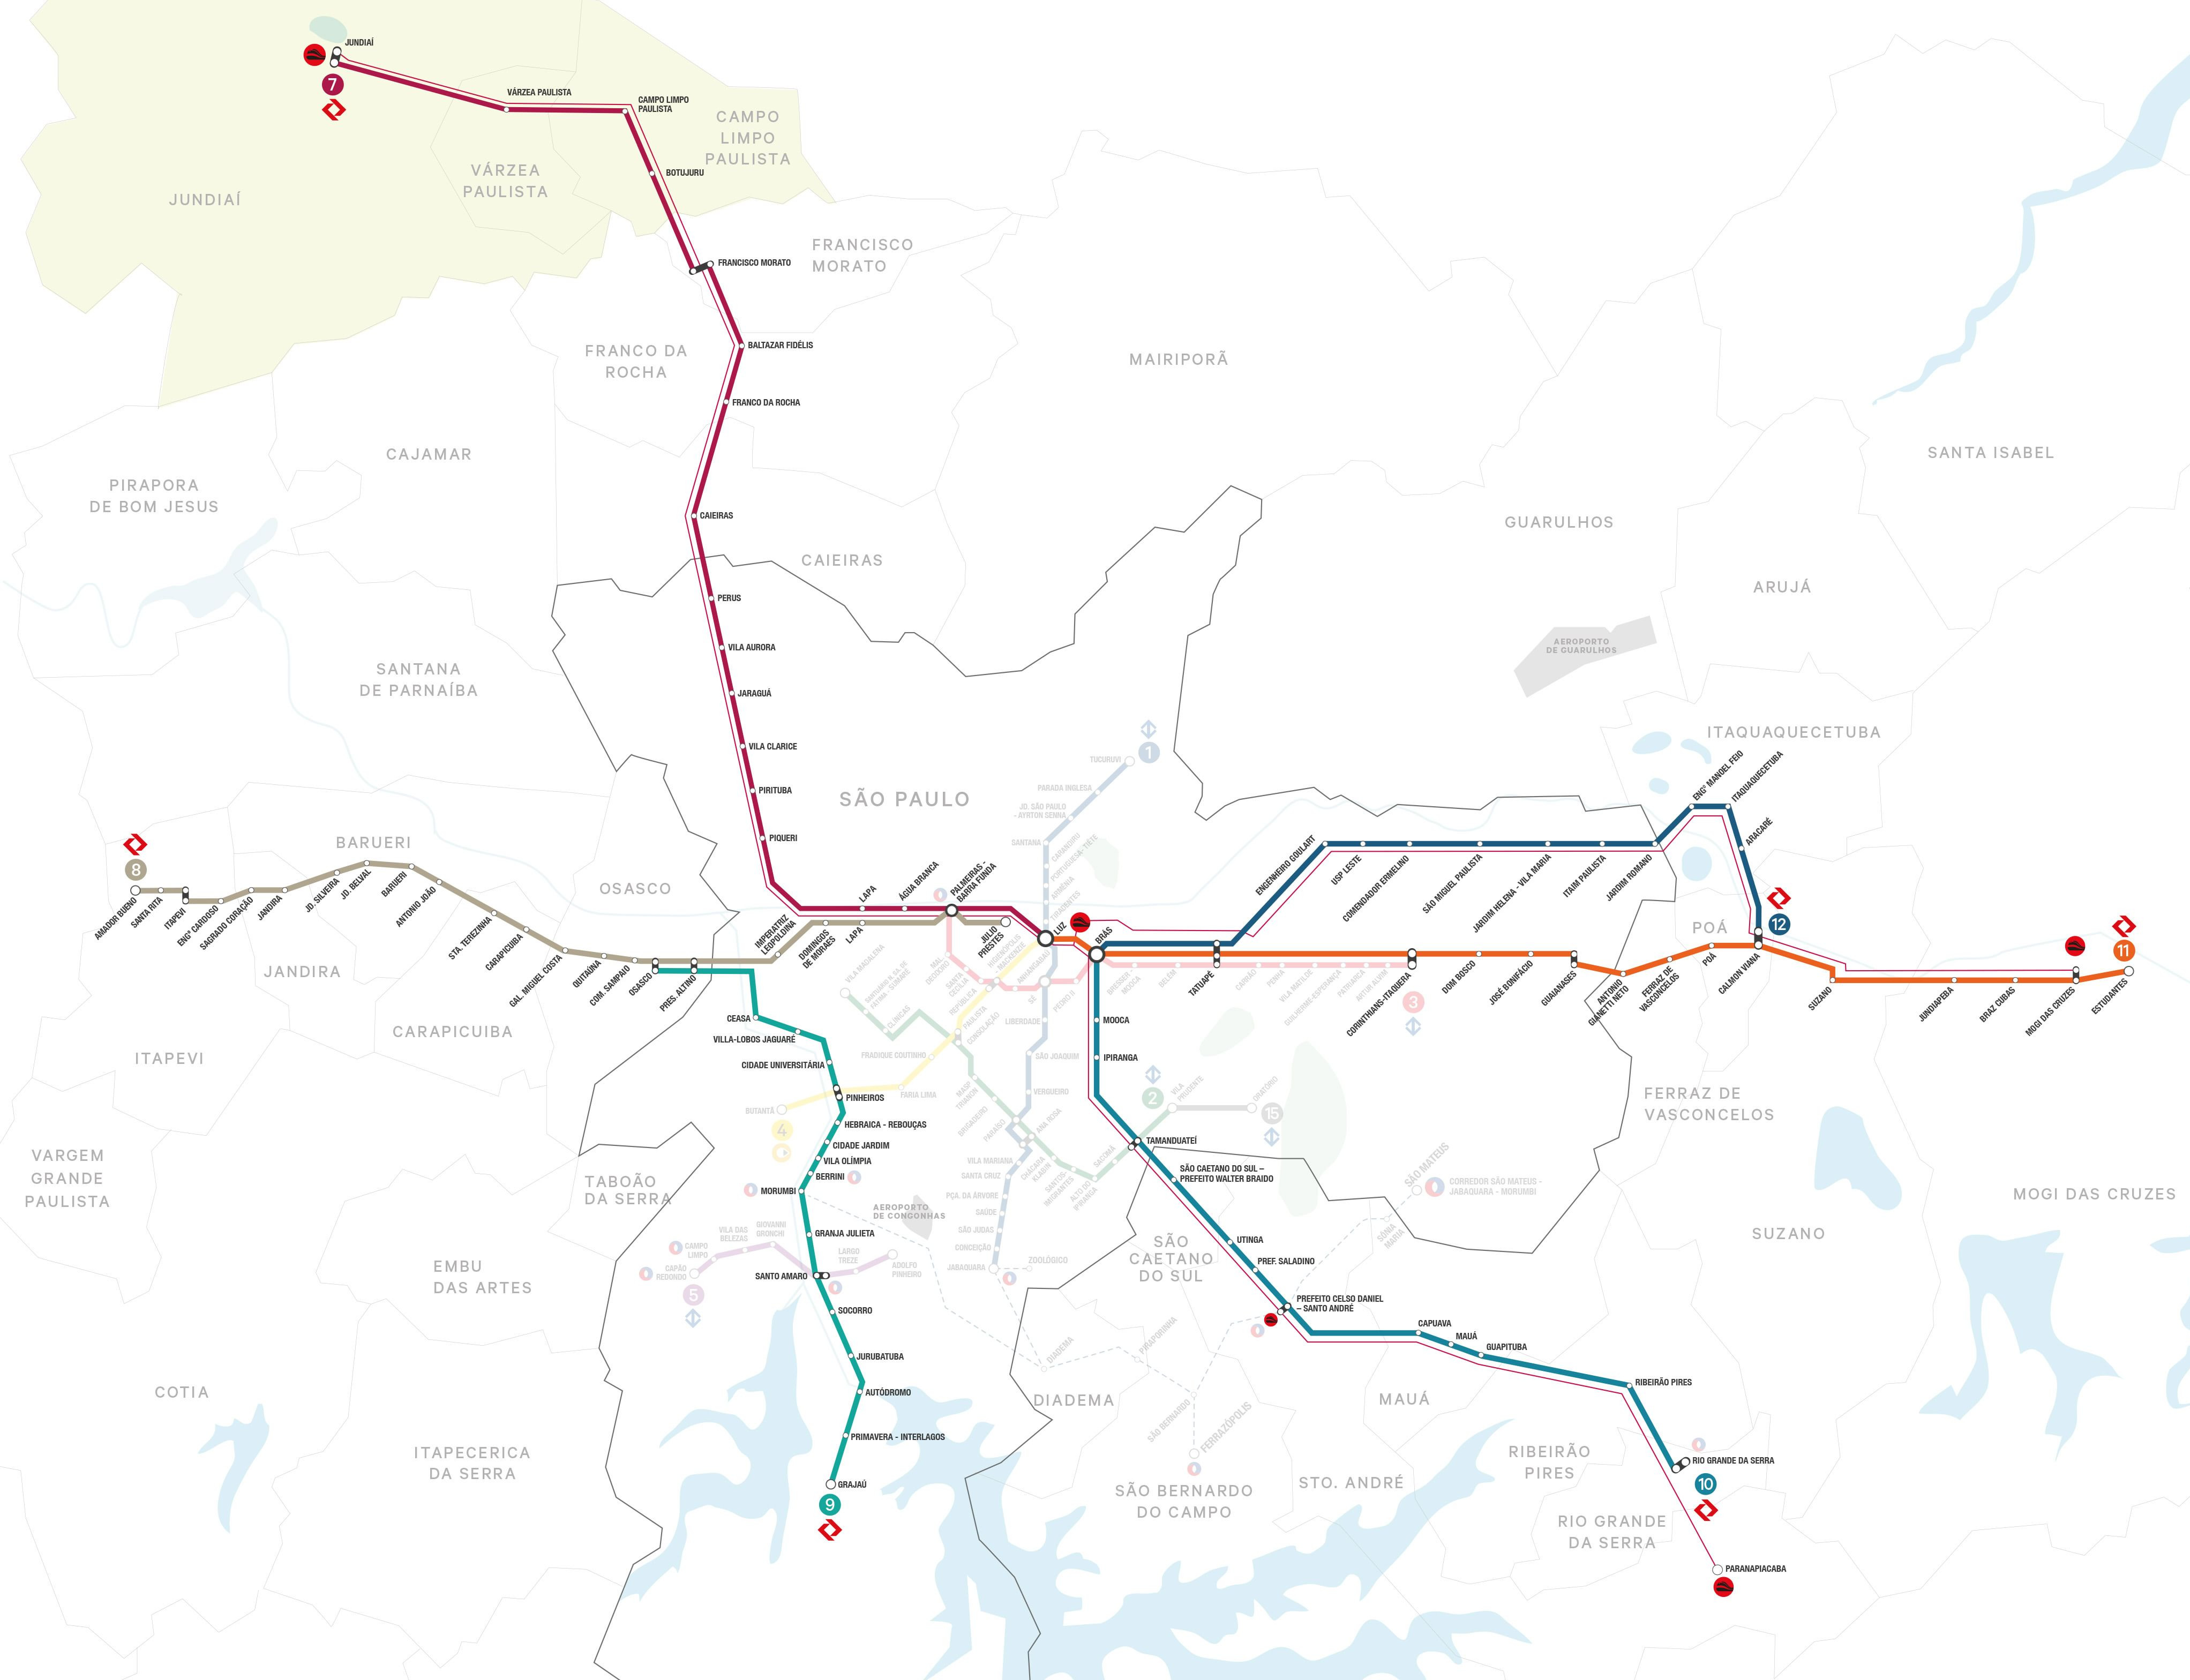
\includegraphics[keepaspectratio,width=7cm]{img_cptm_linhas_crop.jpg}
	\end{figure}
	
\end{frame}

% ----------------- NOVO SLIDE --------------------------------

\begin{frame}{Demanda}
	
	\begin{center}
		\begin{tikzpicture}[scale=0.9, transform shape]
		\begin{axis}[
		title=Gráfico de demanda das seis linhas baseado em \citeonline{sitecptm1},
		grid=both,
		ymin=150,
		ymax=750,
		ybar,
		symbolic x coords={7,8,9,10,11,12},
		nodes near coords, nodes near coords align={vertical},
		xlabel=Linha,
		ylabel=Passageiros (MDU em milhares),
		enlargelimits=0.15,
		]
		\addplot+[ybar] coordinates
		{(7,468.000)
			(8,461.900)
			(9,567.300)
			(10,355.600)
			(11,701.200)
			(12,248.700)};
		\end{axis}
		\end{tikzpicture}
	\end{center}
	
\end{frame}

% ----------------- NOVO SLIDE --------------------------------

\begin{frame}{Abrangência do trabalho}
	
	Das 92 estações totais do sistema, 56 delas se inserem no contexto deste trabalho (60,9\% de toda a malha), onde apenas 11 serão abordadas de forma mais ou menos direta (12\% de toda a malha de todas as estações, 19,6\% inseridas no contexto), dependendo do assunto. Quanto às 11 estações, com base em \citeonline{sitecptm2}, temos o seguinte quadro:
	
	\begin{itemize}
		\item Osasco: 1 de 4 estações (25\%)
		\item Carapicuíba: 0 de 2 estações (0\%)
		\item Barueri: 2 de 4 estações (50\%)
		\item São Paulo: 5 de 46 estações (10,9\%)
	\end{itemize}

\end{frame}

% ----------------- NOVO SLIDE --------------------------------
\section{Fio-condutor}

\begin{frame}{Linha 8 - Motivação}

	\begin{block}{Observação}
		A Linha 8-Diamante é o primeiro dos três casos abordados no trabalho.
	\end{block}

	\vspace*{1cm} 
	
	Motivos da escolha da Linha 8-Diamante:

	\begin{itemize}
		\item Permite uma oportuna exploração da fragmentação urbana provocada por Alphaville
			\begin{itemize}
				\item Linha que corre paralela, ainda que não adjacente, ao empreendimento
				\item Parte do empreendimento fácil de visualizar no trecho compreendido pelas estações Carapicuíba e Barueri	
				\item O ``diálogo'' com a linha só se dá por meio dos ônibus municipais (de Barueri) e intermunicipais (da EMTU)
			\end{itemize}
	\end{itemize}

\end{frame}

% ----------------- NOVO SLIDE --------------------------------

\begin{frame}{Linha 8 - Escopo}

	Estações analisadas:

	\begin{itemize}
		\item General Miguel Costa (divisa de Osasco com Carapicuíba)
		\item Antônio João (divisa de Barueri com Carapicuíba)
		\item Barueri (estação central do município homônimo)
	\end{itemize}
	
\end{frame}

% ----------------- NOVO SLIDE --------------------------------

\begin{frame}{Linha 8 - Demanda}
	
	\begin{center}
		\begin{tikzpicture}[scale=0.8, transform shape]
		\begin{axis}[
		title=Evolução da demanda baseado em Mídia CPTM,
		grid=both,
		scaled ticks=false, tick label style={/pgf/number format/fixed},
		x tick label style={/pgf/number format/1000 sep=},
		y tick label style={/pgf/number format/.cd, set thousands separator={.}},
		legend style={at={(0.5,-0.3)},anchor=north,legend columns=-1},
		ylabel=Passageiros (MDU em milhares),
		xlabel=Ano,
		]
		\addplot coordinates
		{(2011,16275) (2012,16606) (2013,17685) (2014,18838) (2015,18150)};
		\addlegendentry{General Miguel Costa}
		
		\addplot coordinates
		{(2011,7943) (2012,8037) (2013,9187) (2014,11218) (2015,12127)};
		\addlegendentry{Antônio João}	
		
		\addplot coordinates
		{(2011,21302) (2012,21377) (2013,22892) (2014,24205) (2015,23940)};
		\addlegendentry{Barueri}
		
		\end{axis}
		\end{tikzpicture}
	\end{center}
	
\end{frame}

% ----------------- NOVO SLIDE --------------------------------

\begin{frame}{Linha 8 - Antônio João}
	
	\begin{figure}[h]
		\caption{Estação Antônio João vista a partir do viaduto (2015)}
		\includegraphics[keepaspectratio,width=8cm]{fotos/DSCN8163.JPG}
	\end{figure}
	
\end{frame}

% ----------------- NOVO SLIDE --------------------------------

\begin{frame}{Linha 8 - Antônio João}
	
		\begin{figure}[h]
			\caption{Escada metálica que dá acesso ao viaduto (2015)}
			\includegraphics[keepaspectratio,width=8cm]{fotos/DSCN8156.JPG}
		\end{figure}
	
\end{frame}

% ----------------- NOVO SLIDE --------------------------------

\begin{frame}{Linha 8 - Antônio João}
	
		\begin{figure}[h]
			\caption{CSU CardSystem, vizinha da estação (2015)}
			\includegraphics[keepaspectratio,width=8cm]{fotos/DSCN8166.JPG}
		\end{figure}
	
\end{frame}

% ----------------- NOVO SLIDE --------------------------------

\begin{frame}{Linha 8 - Antônio João}
	
	Quando da chegada da CSU em 2009, suas instalações na época foram alardeadas como sendo as do maior \textit{call center} da América Latina\cite{investesp}.
	
\end{frame}

% ----------------- NOVO SLIDE --------------------------------

\begin{frame}{Linha 8 - Antônio João}
		
		\begin{figure}[h]
			\caption{Parque Shopping Barueri, vizinho da estação (2015)}
			\includegraphics[keepaspectratio,width=8cm]{fotos/DSCN8178.JPG}
		\end{figure}
	
\end{frame}

% ----------------- NOVO SLIDE --------------------------------

\begin{frame}{Linha 8 - Antônio João}
	
	Parque Shopping Barueri, inaugurado em novembro de 2011, conta com uma Área Bruta Locável (ABL) de 34,4 mil m$^2$ \cite{valoreconomico}.
	
\end{frame}

% ----------------- NOVO SLIDE --------------------------------

\begin{frame}{Linha 8 - Antônio João}
	
		\begin{figure}[h]
			\caption{Alphaville observado a partir do viaduto (2015)}
			\includegraphics[keepaspectratio,width=8cm]{fotos/DSCN8173.JPG}
		\end{figure}
	
\end{frame}

% ----------------- NOVO SLIDE --------------------------------

\begin{frame}{Linha 8 - Antônio João}
	
	\begin{figure}[h]
		\caption{Linha T245VP1, trajeto estação-Alphaville (2015)}
		\includegraphics[keepaspectratio,width=8cm]{fotos/DSCN8165.JPG}
	\end{figure}
	
\end{frame}

% ----------------- NOVO SLIDE --------------------------------

\begin{frame}{Linha 8 - Relacionando com Henri Acselrad}
	
	Conforme \citeonline[pág. 31]{Acselrad}:``A fragmentação por baixo, sugere-nos \citeonline{Jaglin}, decorre de uma concepção comunitarista de solidariedade, que promove um parcelamento gestionário dos bairros pobres, uma descontinuidade física das redes de ilhas selecionadas de atendimento, gerando competição entre as comunidades e no interior das mesmas por recursos escassos. A fragmentação pelo alto, por sua vez, reúne todas as formas de dessolidarização entre áreas ricas e áreas pobres, de renúncia ao compartilhamento fiscal, tarifário e de redes de infra-estrutura, além das práticas de auto-segregação espacial, via condomínios fechados, gradeamento, segurança privada etc''.

\end{frame}

% ----------------- NOVO SLIDE --------------------------------

\begin{frame}{Linha 8 - Se há diálogo, é para reforçar a segregação}
	
	A auto-segregação espacial e a renúncia à infraestrutura ferroviário de transporte metropolitano é um traço indissociável do que Alphaville representa, estabelecendo um diálogo direto com a Linha 8 da CPTM, não pela articulação direta do empreendimento, como apontei acima, mas pela fragmentação que ele provoca ao não adotá-la, procurando constituir um espaço apartado do restante do município de Barueri.

\end{frame}

% ----------------- NOVO SLIDE --------------------------------

\begin{frame}{Linha 8 - Nem todos os muros são físicos}
	
	Como um importante polo comercial, empresarial e industrial, Alphaville demanda muita mão de obra, sendo que a maioria dos trabalhadores não mora nos residenciais fechados, conclusão talvez óbvia, mas que fica reforçada pelo periódico britânico The Guardian, segundo o qual Alphaville é um dos dez maiores muros do planeta\cite{muro}.

\end{frame}

% ----------------- NOVO SLIDE --------------------------------

\begin{frame}{Linha 8 - General Miguel Costa}
	
	\begin{figure}[h]
		\caption{Visão geral da estação (2015)}
		\includegraphics[keepaspectratio,width=8cm]{fotos/DSCN8237.JPG}
	\end{figure}
	
\end{frame}

% ----------------- NOVO SLIDE --------------------------------

\begin{frame}{Linha 8 - General Miguel Costa}
	
	\begin{figure}[h]
		\caption{Novo terminal metropolitano Km 21 da EMTU (2015)}
		\includegraphics[keepaspectratio,width=8cm]{fotos/DSCN8264.JPG}
	\end{figure}
	
\end{frame}

% ----------------- NOVO SLIDE --------------------------------

\begin{frame}{Linha 8 - Mais facetas de Alphaville}
	
	\begin{exampleblock}{}
		Com um contingente de 154.606 trabalhadores, Alphaville tem um número três vezes menor de moradores, 43.521. Os índices econômicos da população fixa são superlativos: $76,3$\% dos domicílios possuem renda mensal acima de 11.000 reais; em São Paulo são $16,7$\%. A média é de 16.724 reais -- contra 3.427 reais da capital, segundo dados da Cognatis Geomarketing.
		\cite{poloadm}
	\end{exampleblock}
	
\end{frame}

% ----------------- NOVO SLIDE --------------------------------

\begin{frame}{Linha 8 - Comparação oportuna}
	
	Os dados populacionais (tanto da população fixa, como também da população flutuante) de Alphaville tornam oportuna uma rápida comparação com a população das outras cidades.
	
	\begin{itemize}
		\item Osasco: 666.740 habitantes, território com 64.954 km$^2$\cite{ibgeOSA}
		\item Carapicuíba: 369.584 habitantes, território com 34.546 km$^2$\cite{ibgeCPB}
		\item Barueri: 240.749 habitantes, território com 65.701 km$^2$\cite{ibgeBRU}
	\end{itemize}
	
\end{frame}

% ----------------- NOVO SLIDE --------------------------------

\begin{frame}{Linha 8 - General Miguel Costa}
	
	\begin{figure}[h]
		\caption{Sinalização provisória (ou improvisada) (2015)}
		\includegraphics[keepaspectratio,width=8cm]{fotos/DSCN8295.JPG}
	\end{figure}
	
\end{frame}

% ----------------- NOVO SLIDE --------------------------------

\begin{frame}{Linha 8 - General Miguel Costa}
	
	\begin{figure}[h]
		\caption{Embarque sem infraestrutura (2015)}
		\includegraphics[keepaspectratio,width=8cm]{fotos/DSCN8320.JPG}
	\end{figure}
	
\end{frame}

% ----------------- NOVO SLIDE --------------------------------

\begin{frame}{Linha 8 - Desarticulação proposital}
	
	\begin{exampleblock}{}
		A implantação de Alphaville foi favorecida pela abertura da Rodovia Castello Branco, que possibilitou a ligação do empreendimento ao vetor sudoeste da capital.
		
		Ainda hoje, não há uma ligação com o trem metropolitano da CPTM ou um sistema de transporte público eficaz capaz de conectar Alphaville à capital, e mesmo aos municípios do entorno. Pode-se dizer que o elemento estruturador de Alphaville/Tamboré é o viário. Um conjunto de vias mal hierarquizadas conecta os diversos setores do empreendimento: industrial, empresarial, comercial e residencial.
		\cite[pág. 125]{Falcone}
	\end{exampleblock}
	
\end{frame}

% ----------------- NOVO SLIDE --------------------------------

\begin{frame}{Linha 8 - Barueri}
	
	\begin{figure}[h]
		\caption{Estação Barueri, a única modernizada (2016)}
		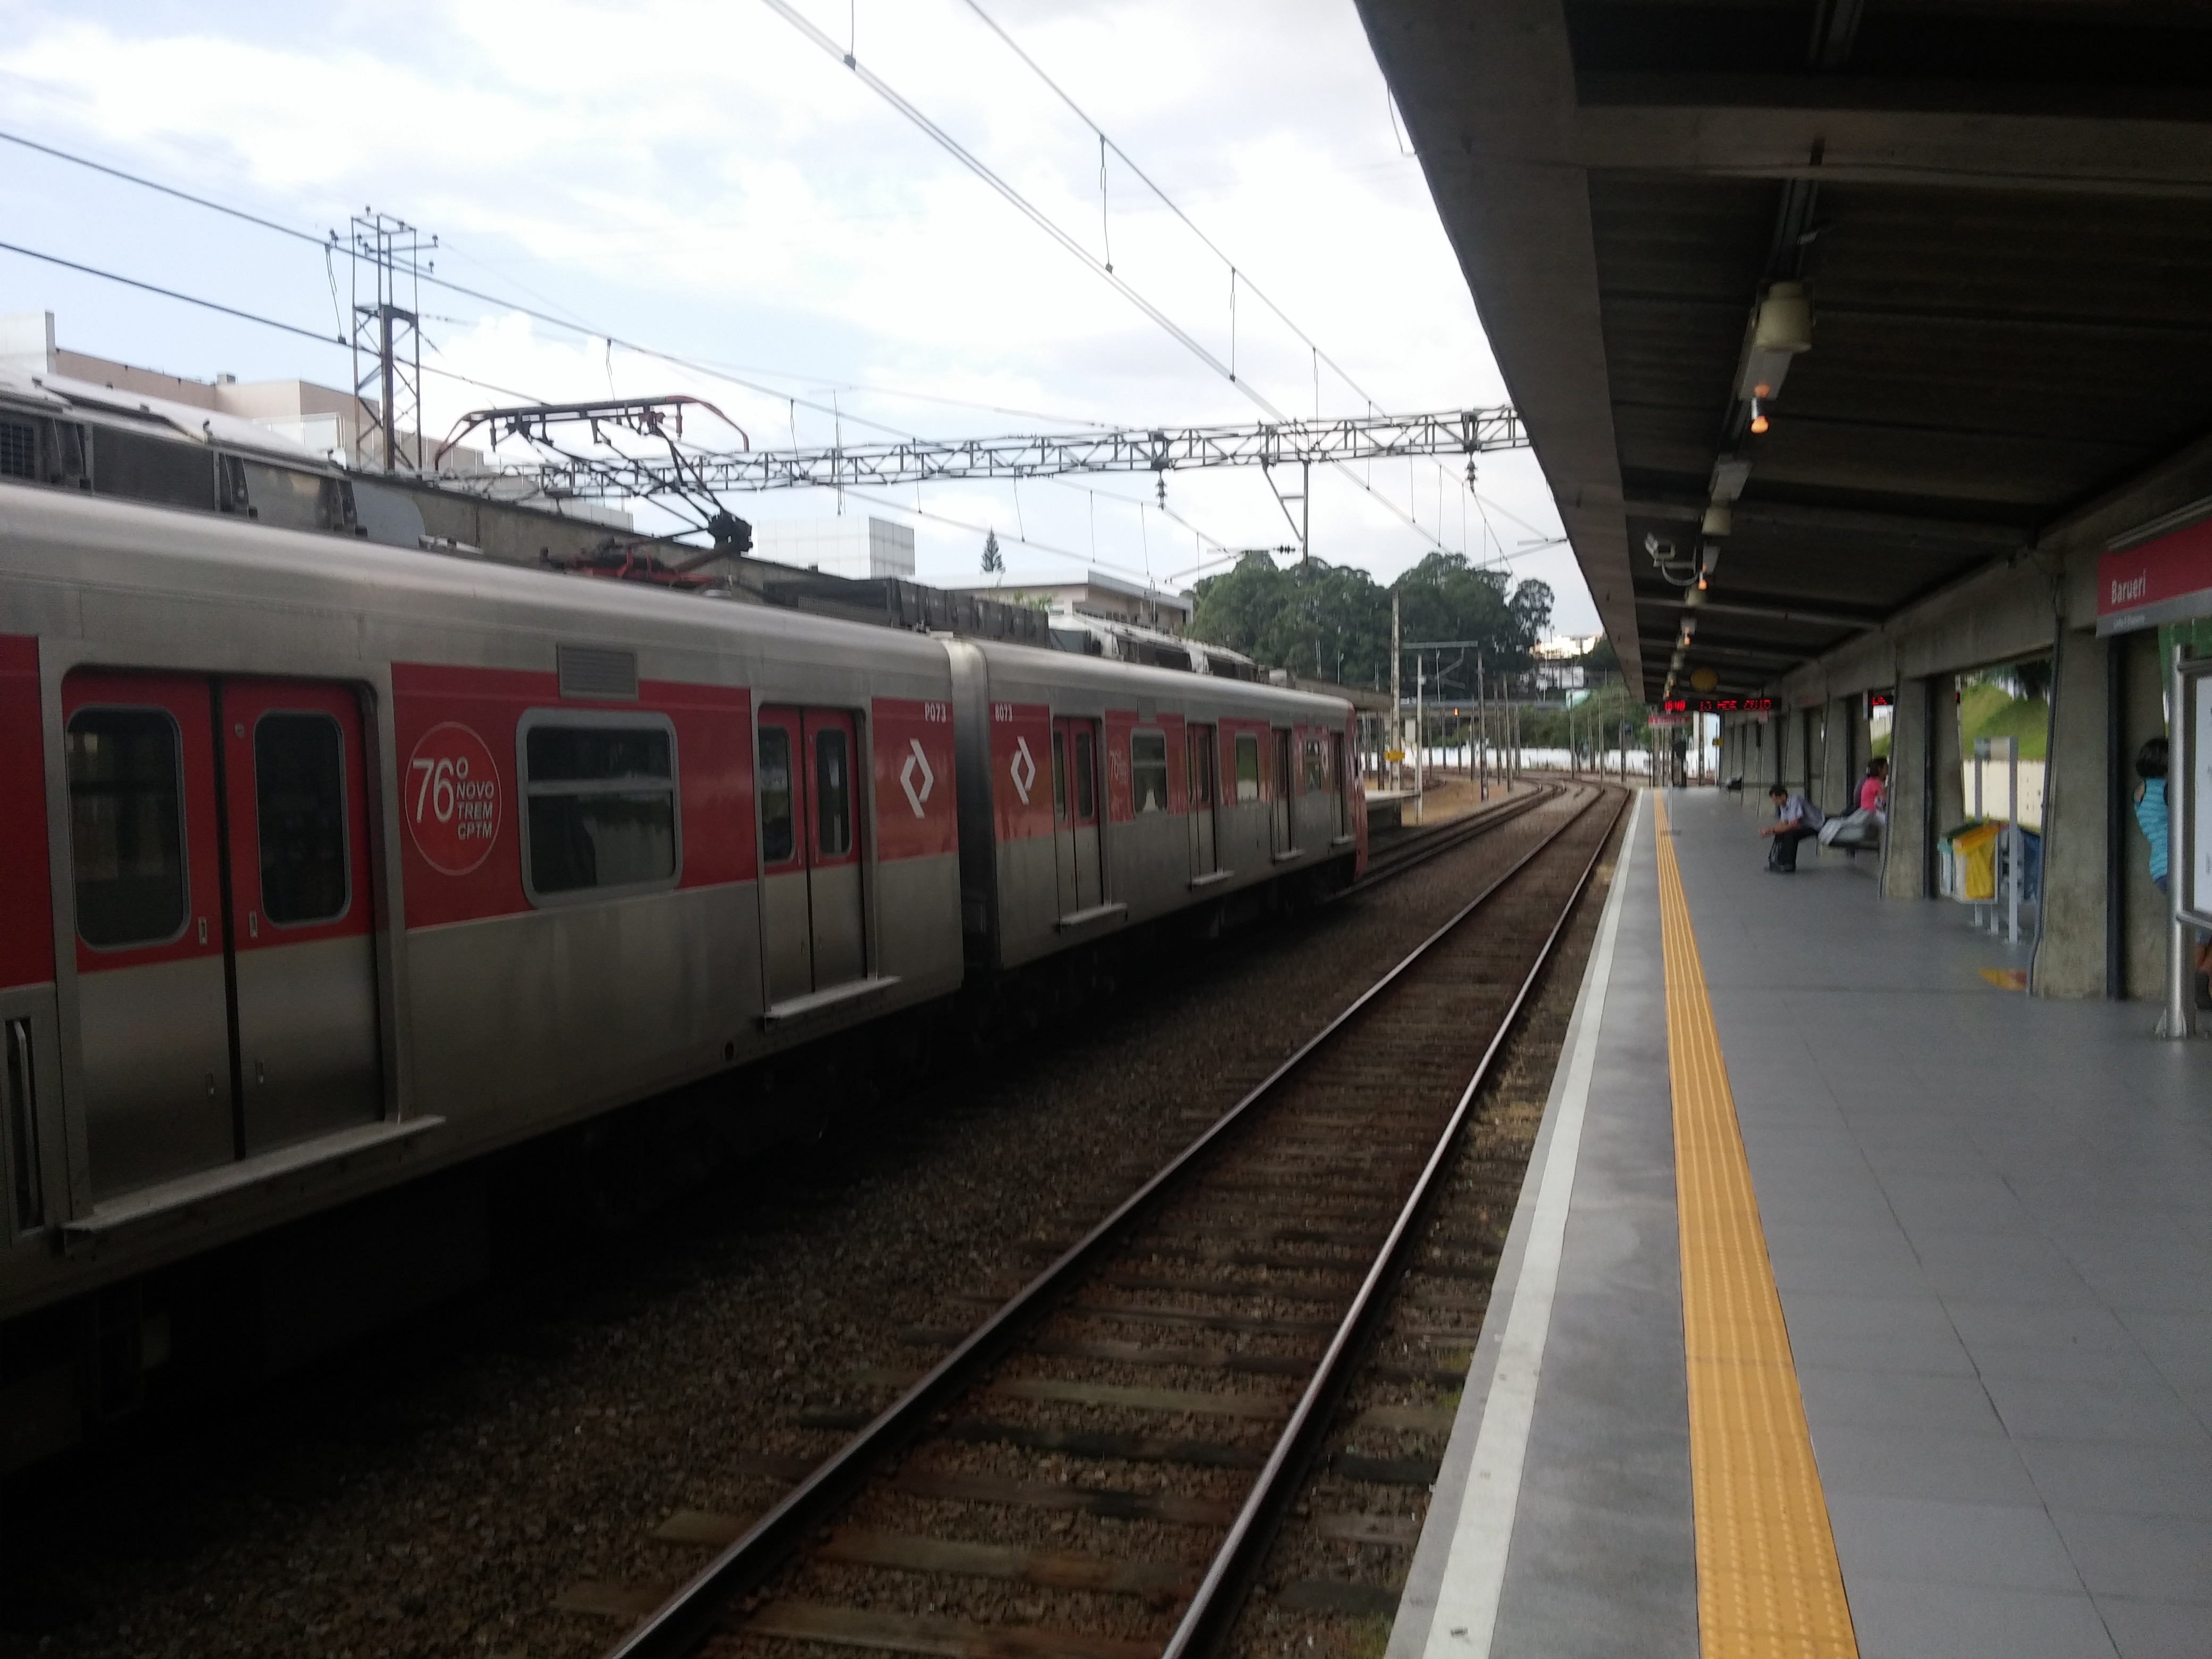
\includegraphics[keepaspectratio,width=8cm]{fotos/20160413_154933_HDR.jpg}
	\end{figure}
	
\end{frame}

% ----------------- NOVO SLIDE --------------------------------

\begin{frame}{Linha 8 - Barueri}
	
	\begin{figure}[h]
		\caption{Terminal fronteiriço à estação (2016)}
		\includegraphics[keepaspectratio,width=8cm]{fotos/20160413_153548.jpg}
	\end{figure}
	
\end{frame}


% ----------------- NOVO SLIDE --------------------------------

\begin{frame}{Linha 8 - Barueri}
	
	\begin{figure}[h]
		\caption{T253VP1, frota com ar condicionado (2016)}
		\includegraphics[keepaspectratio,width=8cm]{fotos/20160413_152547.jpg}
	\end{figure}
	
\end{frame}
% ----------------- NOVO SLIDE --------------------------------

\section{Conclusão}

\begin{frame}{Conclusão}
	
	\begin{itemize}
	\item Pude ``costurar'' melhor alguns conceitos apresentados pela disciplina, de forma a garantir sua fixação com a aplicação deles em situações presentes numa parcela da infraestrutura abordada.
	\item Foi possível estabelecer relações para além da bibliografia básica, mas sempre mantendo a transversalidade.
	\item Necessidade de estruturar melhores políticas públicas que recuperem, em totalidade, o potencial estruturante da ferrovia, ao mesmo tempo que garantam a sobrevivência das mesmas políticas com base na infraestrutura que lhes servirá de justificativa em primeiro lugar.
	\item Heterogeneidade não só da capital ou da RMSP. mas da própria malha do Trem Metropolitano.
	\end{itemize}

\end{frame}

% ----------------- NOVO SLIDE --------------------------------

\section{Referências}

% --- O comando \allowframebreaks ---
% Se o conteúdo não se encaixa em um quadro, a opção allowframebreaks instrui 
% beamer para quebrá-lo automaticamente entre dois ou mais quadros,
% mantendo o frametitle do primeiro quadro (dado como argumento) e acrescentando 
% um número romano ou algo parecido na continuação.

\begin{frame}[allowframebreaks]{Referências}
	\bibliography{referencias}
\end{frame}

% ----------------- FIM DO DOCUMENTO -----------------------------------------
\end{document}